\documentclass[12pt]{article}
\usepackage{geometry}                % See geometry.pdf to learn the layout options. There are lots.
\geometry{letterpaper}                   % ... or a4paper or a5paper or ... 
%\geometry{landscape}                % Activate for for rotated page geometry
\usepackage[parfill]{parskip}    % Activate to begin paragraphs with an empty line rather than an indent
\usepackage{daves,fancyhdr,natbib,graphicx,dcolumn,amsmath,lastpage,url}
\usepackage{amsmath,amssymb,epstopdf,longtable}
\usepackage{paralist} 
\DeclareGraphicsRule{.tif}{png}{.png}{`convert #1 `dirname #1`/`basename #1 .tif`.png}
\pagestyle{fancy}
\lhead{CE 3372 -- Water Systems Design}
\rhead{FALL 2017}
%\rhead{SPRING 2016}
%\rhead{FALL 2011}
%\rhead{SPRING 2012}
%\rhead{FALL 2012}
%\rhead{FALL 2015}
%\rhead{FALL 2010}
%\lfoot{EXERCISE 1 -- REVISION 1}
%\lfoot{EXERCISE 1 -- REVISION 2}
%\lfoot{EXERCISE 1 -- REVISION 3}
%\lfoot{EXERCISE 1 -- DUE 26 JAN 2012}
%\lfoot{EXERCISE 1 -- DUE 4 SEP 2012}
\lfoot{EXERCISE 17}
\cfoot{}
\rfoot{Page \thepage\ of \pageref{LastPage}}
\renewcommand\headrulewidth{0pt}
\newcommand\tab[1][1cm]{\hspace*{#1}}


\begin{document}
\begin{center}
{\textbf{{ CE 3372 -- Water Systems Design} \\ {Exercise Set 17}}}
\end{center}
\begingroup
\begin{tabular}{p{1in} p{5in}}
Purpose: & Sewer system pipe alignment in SWMM \\

\end{tabular}
\endgroup
\section*{\small{Exercises}}
\begin{enumerate}

%%%%%%%%%%%%%%%%%%%%%%%%%%%%%%%%%%%%%%%%%%%%%%%%%%%%%%%%%%%%%%%%%%%%%%%%%%%%%%
\item Figure \ref{fig:SWMMCases} is a sketch of four different configurations.  All pipes have Manning's n $0.015$.  The invert elevations, pipe diameters, and pipe lengths are given on the sketch.   The input flows are $Q_1 = 20 \text{ CFS}$, $Q_2 = 66 \text{ CFS}$, $Q_3 = 110 \text{ CFS}$, at the indicated nodes.   The upper two cases have a \texttt{FREE} outfall downstream boundary condition; the lower two cases have a \texttt{FIXED} pool elevation boundary condition (pool elevation is $3.5$ feet).

\begin{figure}[h!] %  figure placement: here, top, bottom, or page
\centering
   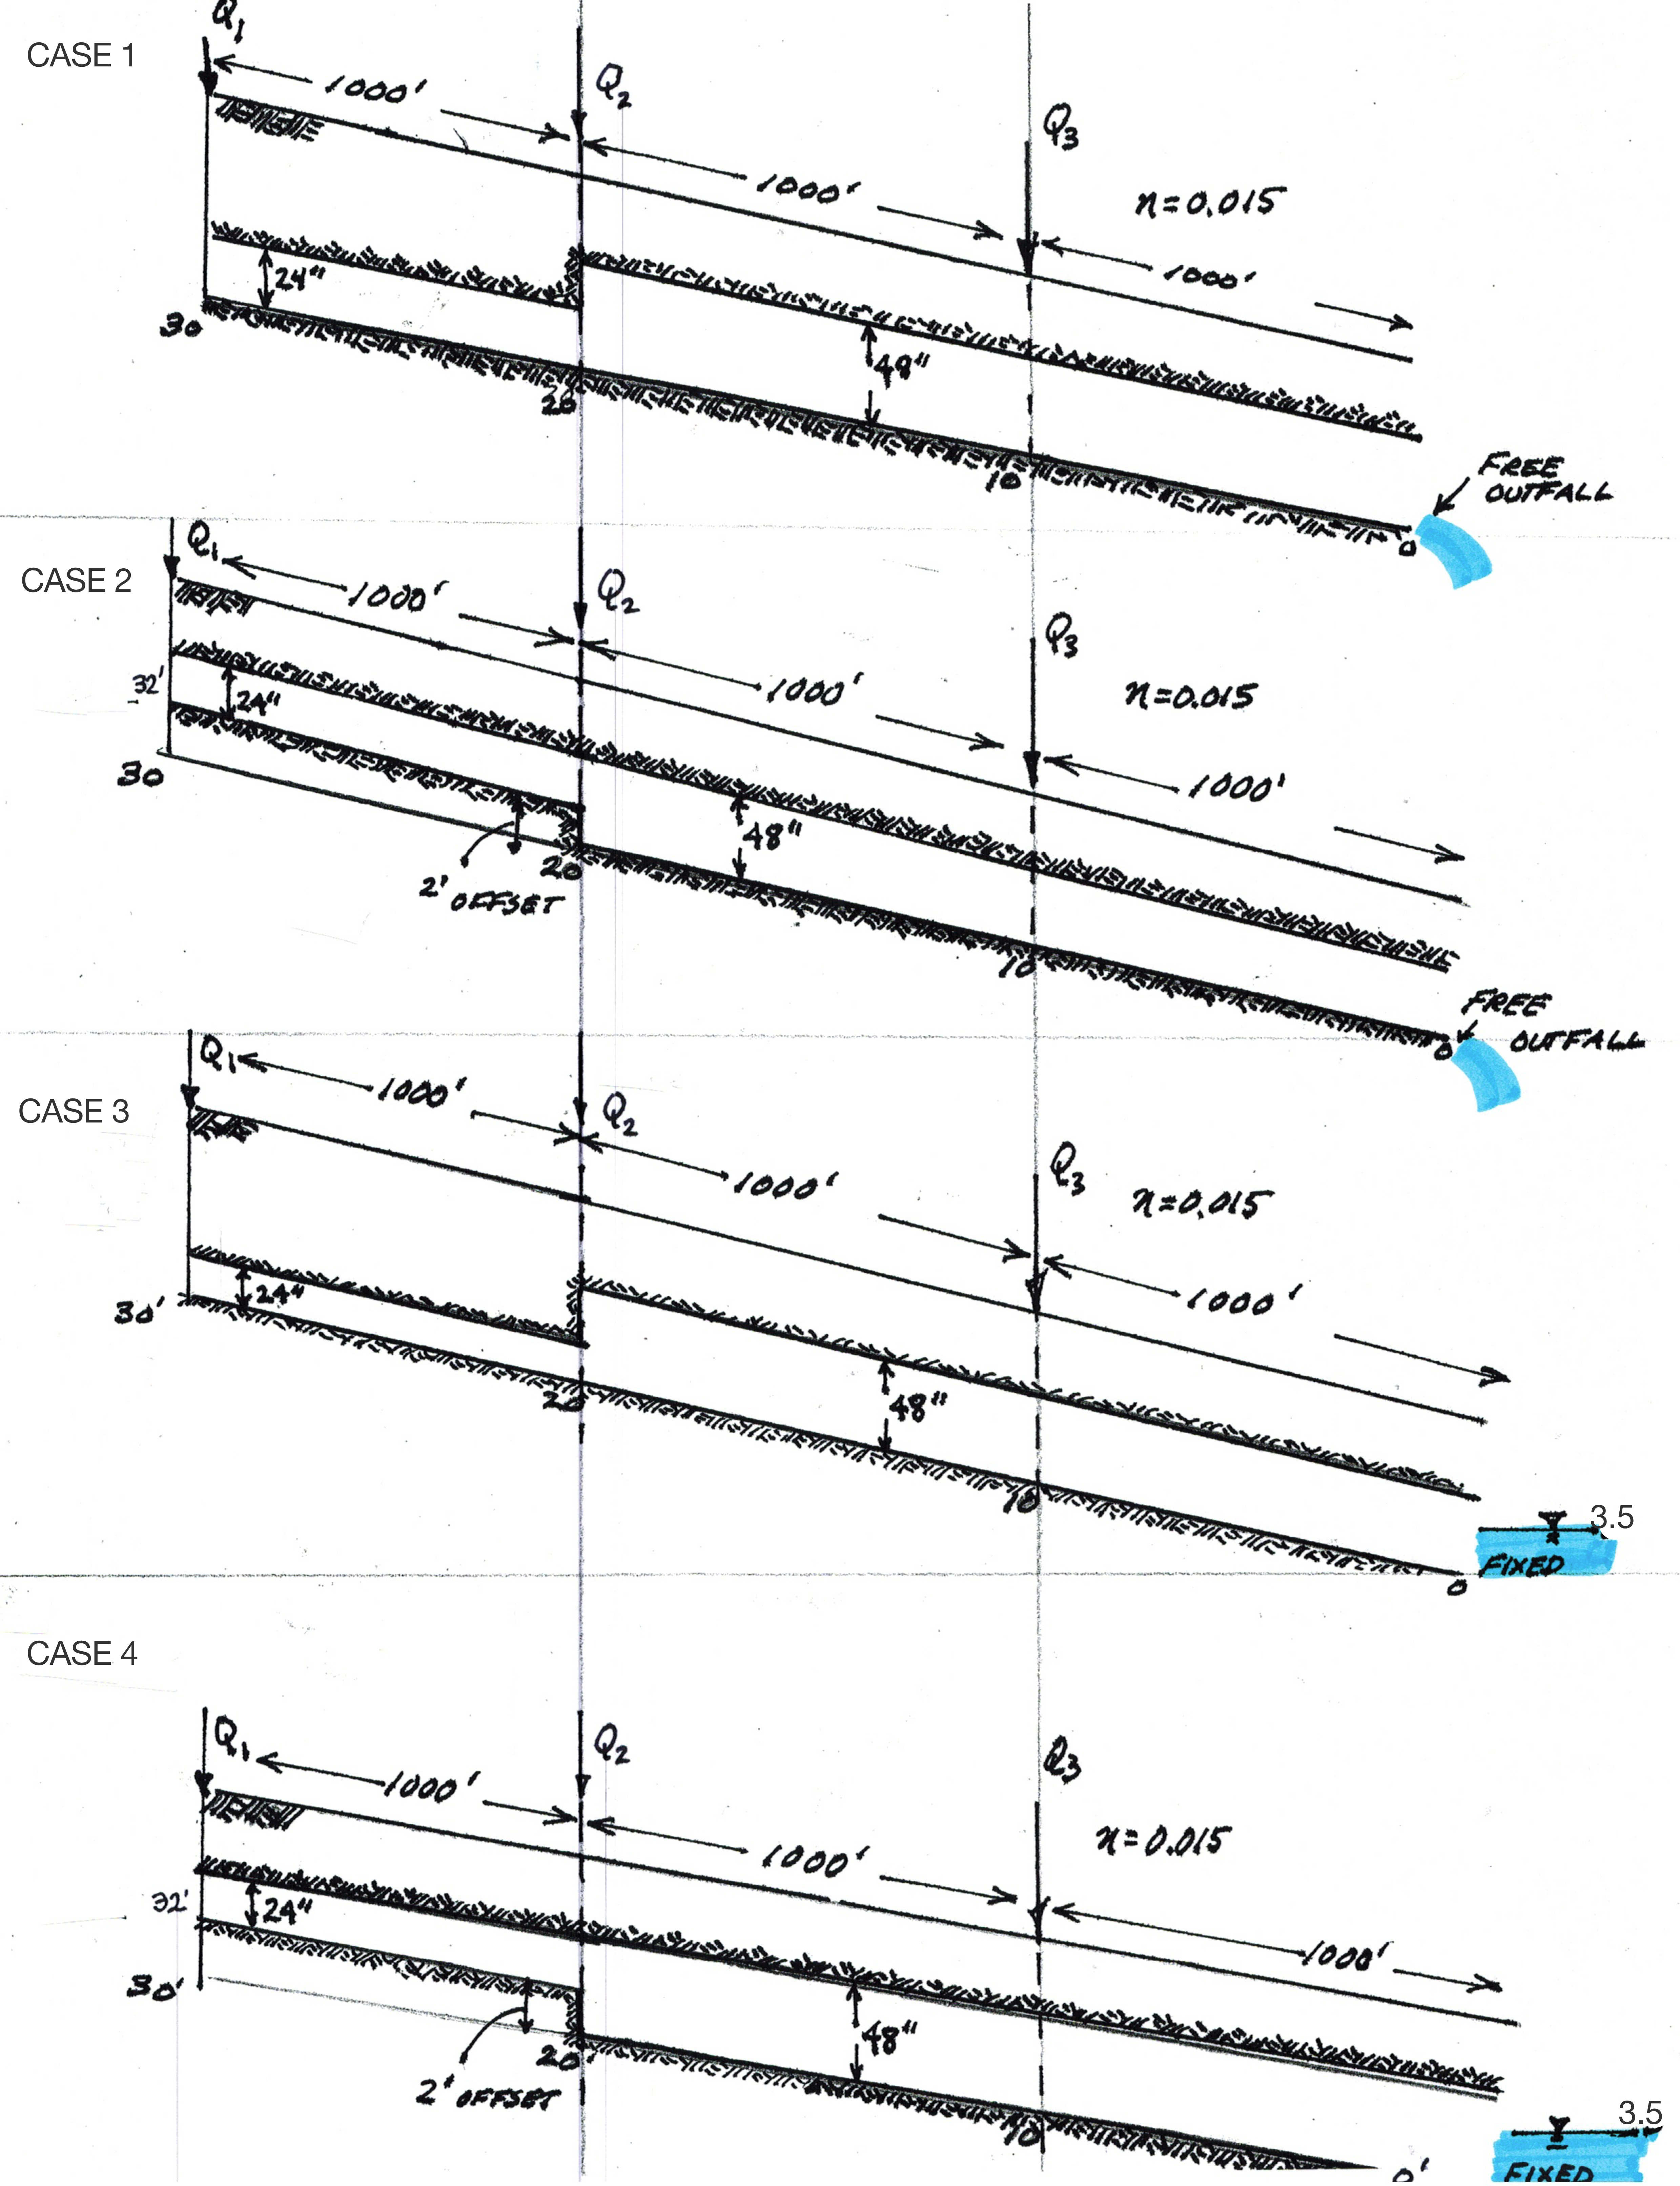
\includegraphics[width=5in]{SWMMCases.jpg}
   \caption{Four (4) cases to model in SWMM}
   \label{fig:SWMMCases} 
\end{figure}


Build a SWMM model that implements the four cases.  Once the model is functional, run the model for a 6-hour interval using \texttt{DYNAMIC WAVE} routing, and use the output conditions at hour 6 of the simulation to address the following list of tasks/questions.  Assume that the maximum depth at each \textbf{node} is 15 feet.

\begin{enumerate}[a)]
\item For Case 1 (Upper most condition), screen capture the profile plot. 
\item Which of the pipes in Case 1 are surcharged? 
\item What is the computed discharge in each pipe (from left to right)? 
\item For Case 2 (Second from top condition), screen capture the profile plot. 
\item Which of the pipes in Case 2 are surcharged? 
\item What is the computed discharge in each pipe (from left to right)? 
\item Does Case 2 have more unused capacity than Case 1? 
\item For Case 3 (Second from bottom condition), screen capture the profile plot. 
\item Which of the pipes in Case 3 are surcharged? 
\item What is the computed discharge in each pipe (from left to right)?
\item For Case 4 (Bottom condition), screen capture the profile plot.
\item Which of the pipes in Case 4 are surcharged? 
\item What is the computed discharge in each pipe (from left to right)? 
\item Does Case 4 have more unused capacity than Case 3? 
\item Explain the hydraulic advantage of matching the soffit (crown) elevations in contrast to matching the flow line (invert) elevations at a pipe diameter change.
\end{enumerate}
\end{enumerate}

%\begin{thebibliography}{}
%
%\bibitem[\protect\citeauthoryear{Swamee and Jain}{Swamee and Jain}{1976}]{jain1976}
%Swamee and Jain, A. K., 1976. Explicit equations for pipe-flow problems.  ASCE J. of Hyd. Div., 102(HY5) pp. 657-664 
%
%
%\end{thebibliography}


\end{document}  